\documentclass{article}

\usepackage[utf8]{inputenc}
\usepackage[T1]{fontenc}
\usepackage{lipsum}
\usepackage{graphicx}
\usepackage{amsmath}
\usepackage[margin=1in]{geometry}
\usepackage{titlesec}
\usepackage{graphicx}
\usepackage{floatflt,epsfig}
\usepackage[utf8]{inputenc}
\usepackage[T1]{fontenc}
\usepackage{lipsum}
\usepackage{graphicx}
\usepackage{amsmath}
\usepackage[margin=1in]{geometry} 
\usepackage{titlesec}
\usepackage{listings}
\usepackage{xcolor}

\lstdefinelanguage{XML}
{
  morestring=[b]",
  morestring=[s]{>}{<},
  morecomment=[s]{<?}{?>},
  morecomment=[s][\color{green!50!black}]{<!--}{-->},
  stringstyle=\color{blue},
  identifierstyle=\color{red},
  keywordstyle=\color{orange},
  commentstyle=\color{green!50!black},
  basicstyle=\small\ttfamily,
  frame=single, 
  breaklines=true,
  breakatwhitespace=true,
  tabsize=2,
  showstringspaces=false,
  captionpos=b,
}

\lstdefinelanguage{Java}{
  keywords={abstract,assert,boolean,break,byte,case,catch,char,class,const,continue,default,do,double,else,enum,extends,false,final,finally,float,for,goto,if,implements,import,instanceof,int,interface,long,native,new,null,package,private,protected,public,return,short,static,strictfp,super,switch,synchronized,this,throw,throws,transient,true,try,void,volatile,while},
  morekeywords={[2]System,out},
  morecomment=[l]{//},
  morecomment=[s]{/*}{*/},
  morestring=[b]",
  basicstyle=\small\ttfamily,
  keywordstyle=\color{blue}\bfseries,
  keywordstyle={[2]\color{orange}\bfseries},
  commentstyle=\color{green!70!black},
  stringstyle=\color{red},
  showstringspaces=false,
  tabsize=2,
  breaklines=true,
  breakatwhitespace=true,
  frame=single, 
  captionpos=b
}


\titleformat{\section}
{\LARGE\bfseries}{\thesection}{1em}{}

\titleformat{\subsection}
{\Large\bfseries}{\thesection}{1em}{}

\begin{document}

\pagestyle{empty}

\section*{Intents}
\large

\subsection*{Reminder Activities}
Fino ad ora le nozioni trattate promuovono lo sviluppo di un'applicazione \textit{mono-activity}, uno dei paradigmi più utilizzati all'interno di \textit{Android}, dato soprattutto dall'abuso del metodo \textit{SetContentView()}. Tuttavia, in certe circostanze, potrebbe essere necessario implementare più di una singola attività. Tutto questo si traduce in un ulteriore layer di difficoltà, in quanto le conoscenze possedute non permettono di manipolare un insieme di attività.\vspace*{7pt}\\
Proseguendo, la possibilità di navigare e, pertanto, di gestire molteplici \textit{activity} è data dalla nozione \textbf{intent}. Innanzitutto occorre che l'insieme di \textit{activities} sia dichiarato all'interno del \textit{Manifest}, passo fondamentale affinchè sia possibile correlare le attività, per poi sviluppare gli \textit{intenti}; tuttavia è bene prima soffermarsi sulle peculiarità di questo strumento.

\subsection*{Overview intent}
Un \textit{intent} rappresenta simbolicamente un \textit{collante} tra attività durante \textit{runtime}. Effettivamente è definito come un \textit{oggetto messaggio}, poichè demanda ad Android di compiere determinate azioni rispetto a specifici dati inviati in input. Per cui, dalla breve definizione precedente, un \textit{intent} è in grado di passare dati, chiamare componenti e di utilizzare funzionalità di applicazioni già installate.\vspace*{7pt}\\
Un \textit{intento} è rappresentato graficamente come un bundle contenente informazioni, relative sia al \textit{ricevitore} della comunicazione che al sistema \textit{Android}.
\begin{lstlisting}[language=JAVA, title=Inizializzazione di un intent]
val intent:Intent = Intent();
\end{lstlisting}
Esistono due tipi di \textit{intent}, suddivisi in:
\begin{enumerate}
    \itemsep0em
    \renewcommand*{\labelenumi}{-}
    \item \textbf{Intent explicit}, lo sviluppatore è a conoscenza del \textit{receiver target} del componente demandato
    \item \textbf{Intent implicit}, lo sviluppatore non è a conoscenza del \textit{receiver target} del componente demandato
\end{enumerate}
Per cui, tramite i parametri inviati, il \textit{sistema operativo} riesce a scindere sulla tipologia di \textit{intent}; tutto dipende se sia dichiarato o meno il \textit{Component Name}. Rispetto a quanto detto, susseguono due atteggiamenti distinti da parte del \textit{operating system}, in cui:
\begin{enumerate}
    \itemsep0em
    \renewcommand*{\labelenumi}{-}
    \item Nel primo caso il sistema operativo, interrogando il \textit{Manifest}, è in grado di risalire allo specifico componente, risvegliandolo
    \item Contrariamente, nel secondo caso, l'\textit{operating system} controlla tutte le attività dell'applicazioni installate, deducendo quali fra esse risponda alla richiesta formulata
\end{enumerate}

\subsection*{Intent Description: Explicit}
\textit{Intenti espliciti} possiedono il \textit{Component Name}; si tratta di un tag opzionale, ma all'interno di un ambiente simile la sua dichiarazione diviene obbligatoria.
\begin{lstlisting}[language=JAVA, title=Inizializzazione di un intent]
intent.setComponent(ComponentName(
    this, // riferimento al contesto attuale
    MyActivity::class.java)
)
\end{lstlisting}
Affinchè sia possibile risvegliare una nuova attività, posta all'interno della stessa applicazione, si adotta la sintassi sottostante.
\begin{lstlisting}[language=JAVA, title=Start di una nuova activity]
val intent:Intent = Intent(this, ActivityTwo::class.java)
startActivity(intent)
\end{lstlisting}    
Tramite il metodo \textit{startActivity()} è direttamente imposto che il componente gestito e manipolato dall'\textit{intent} debba essere un'attività.

\subsection*{Intent Description: Implicit}
Come già descritto precedentemente, \textit{intenti impliciti} non sono caratterizzati da un \textit{Component Name}. Questo testimonia un approccio differente rispetto alla propria controparte, in cui Android definisce quali componenti siano associabili all'\textit{intent} specifico. In caso due o più \textit{component} dovessero rispettare le aspettative richieste, sarà compito dell'user decidere quali fra essi debba essere utilizzato.

\subsection*{Field dell'Intent}
Graficamente sono definiti sei field che contraddistinguono un \textit{intent}, indifferentemente dalla tipologia. Di seguito è proposta una breve descrizione di ognuno di essi, omettendo il tag \textit{Component Name}, dato che più volte è stata ribadita la sua nozione.\\
\begin{center}
    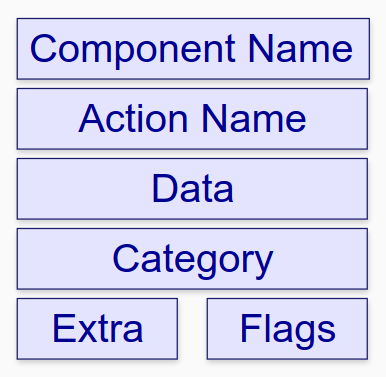
\includegraphics[width=0.25\textwidth]{foto1.png}
\end{center}
\begin{enumerate}
    \itemsep0em
    \renewcommand{\labelenumi}{ }
    \item \textbf{Action Name}, si tratta semplicemente di una stringa nominativa dell'azione in questione. È obbligatoria nel caso di intenti impliciti, definita dallo sviluppatore oppure scelta tra le molteplici già disponibili.
    \begin{lstlisting}[language=JAVA, title=Definizione del field action name]
intent.action = Intent.ACTION_EDIT // action name predefinito
intent.action = "com.example.MyApplication.MY_ACTION" // action name personalizzato
    \end{lstlisting}
    L'impiego del field è attuato qualora si voglia imporre il comportamento che l'\textit{activity} risvegliata debba eseguire
    \item \textbf{Data}, rappresenta i dati passati dal chiamante al ricevitore. La sintassi utilizzata promuove una schema simile a quanto riportato.
    \begin{lstlisting}[language=JAVA, title=Definizone del field data]
intent.data = "https://www.unibo.it/"
intent.type = "text/html"
    \end{lstlisting}
    Prima di proseguire è bene evidenziare alcuni aspetti salienti dei due metodi. Innanzitutto le due funzioni si annullano a vicenda, pertanto qualora si abbia l'opportunità di modificare sia il \textit{name} che il \textit{type}, è necessario usufruire del metodo \textbf{setDataAndType()}. Il \textit{name} coincide con l'\textit{Uniform Resouce Identifier}, mentre il \textit{type} testimonia il \textit{Multipurpose Internet Mail Extensions} 
    \item \textbf{Category}, una stringa che aggiunge delle informazioni all'\textit{action} da eseguire. Tipicamente è riportata in relazione ad \textit{intent} che abbiano ulteriori \textit{features} da considerare nella loro operatività.
    \begin{lstlisting}[language=JAVA, title=Definizone del field category]
intent.addCategory(Intent.CATEGORY_BROWSABLE)
    \end{lstlisting}
    \item \textbf{Extra}, informazioni aggiuntive precisate dal mandante, predisposte secondo la coppia chiave-valore.
    \begin{lstlisting}[language=JAVA, title=Definizone del field extra]
val intent:Intent = Intent(Intent.ACTION_SEND)
intent.putExtra(Intent.EXTRA_MAIL, "federico.montori2@unibo.it")
    \end{lstlisting}
    \textit{Extras} possono essere predefiniti, ciò avviene per la maggiore delle \textit{actions}, le quali richiedono che siano indicate tali informazioni aggiuntive
    \item  \textbf{Flags}, interi contenenti, nuovamente, informazioni aggiuntive che istruiscono \textit{Android} in relazione all'approccio che debba mantenere nei confronti dei componenti risvegliati.
    \begin{lstlisting}[language=JAVA, title=Definizione del field flags]
intent.flags = Intent.FLAG_ACTIVITY_NEW_TASK or
               Intent.FLAG_ACTIVITY_NO_ANIMATION
    \end{lstlisting}
\end{enumerate}

\subsection*{Intent Resolution}
Fino ad ora è stata piu volte ribadita la differenza principale tra un intento \textit{esplicito} ed \textit{implicito}; ciò dipende dal contenuto del bundle che li caratterizza, in cui, tipicamente, il primo citato è adottato qualora il \textit{componente} risvegliato appartenga alla stessa applicazione, mentre nel secondo caso si attua qualora siano necessarie funzionalità provenienti da attività esterne all'applicazione sviluppata.\vspace*{7pt}\\
Tuttavia sorgono alcuni problemi, relativi a due contesti:
\begin{enumerate}
    \itemsep0em
    \renewcommand{\labelenumi}{-}
    \item Come riconoscere quale componente risponda alla richiesta, dato che Android rileva l'attività di destinazione in completa autonomia
    \item Identificare quali componenti possano gestire gli intenti creati
\end{enumerate}
Rispetto alla prima problematica è necessario stabilire un esempio di supporto, definito come segue.
\begin{lstlisting}[language=JAVA, title=Esempio di creazione di un intent implicito]
val intent:Intent = Intent(Intent.ACTION_SEND)
intent.putExtra(Intent.EXTRA_TEXT, "Hello World!")
intent.type = "text/plain"
if(intent.resolveActivity(packageManager) != null) 
    startActivity(intent)

\end{lstlisting}
Si evidenziano alcuni aspetti descritti precedentemente, tra cui \textit{Action Name}, \textit{Extras} ed infine \textit{Data}. Lo sketch di codice rappresenta appieno il quesito posto, in cui non è possibile rilevare quale componente comunichi dati. In tal senso è spesso attuato un paradigma, in cui l'utente è forzato a scegliere il componente che sarà successivamente risvegliato; a livello di codice quest'ultimo passaggio si traduce nell'inizializzazione di una variabile \textbf{chooser}.
\begin{lstlisting}[language=JAVA, title=Inserimento dell'elemento chooser]
val intent:Intent = Intent(Intent.ACTION_SEND)
intent.putExtra(Intent.EXTRA_TEXT, "Hello World!")
intent.type = "text/plain"
val chooser = Intent.createChooser(intent, "You have to choose!")
if(intent.resolveActivity(packageManager) != null) 
    startActivity(chooser)
\end{lstlisting}
Proseguendo, la seconda problematica è inerente al ricevitore della richiesta. Occorre quindi definire quali intenti il componente di riferimento possa gestire; ciò avviene attraverso l'utilizzo del tag \textit{<intent-filter>/</intent-filter>} posto all'interno del \textit{Manifest}.
\begin{lstlisting}[language=XML, title=Inserimento dell'intent-filter nel Manifest]
<activity
    android:name = "MyApplication"
    android:exported = "true"
    <intent-filter>
        <action android:name = "com.example.ACTION_ECHO" />
    </intent-filter>
</activity>
\end{lstlisting}    
Piccola peculiarità, è dettata dalla presenza dell'\textit{attribute} \textit{exported}; esso testimonia che l'\textit{activity} può essere invocata da ulteriori applicazioni. Proprio per tale ragione è necessario esplicitare quali \textit{intents} il componente sia in grado di manipolare.
\end{document}